% =====================================================================
\chapter{Result Analysis}
\label{ch:results}
% =====================================================================

This chapter reports the results of the experiments described in
Chapter~\ref{ch:impl}. It first defines the performance measures, then
analyses the three systems (heuristic-only, transformer-only and the cascade
at three operating points) on accuracy, calibration, generalisation,
robustness, fairness, efficiency and explainability. It closes by assessing
the system against the success criteria of Table~\ref{tab:gap-obj} and the
hypotheses H1--H4 of Chapter~\ref{ch:problem}. All numbers are produced by the
scripts in the \texttt{train/} directory from a single run with random seed 42
and can be regenerated with the commands of Listing~\ref{lst:pipeline}.

% ---------------------------------------------------------------------
\section{Performance Measures}
\label{sec:measures}
% ---------------------------------------------------------------------

\subsection{Confusion Matrix}

Every detector produces, for each document, a probability $p(d)$ and a label
$\hat{y} = \mathbb{1}[p(d) \ge \tau]$ with $\tau = 0.5$. With the AI-generated
class as the positive class, the decisions on a labelled set fall into the four
cells of the confusion matrix (Table~\ref{tab:confusiondef}).

\begin{table}[H]
\caption{Confusion matrix for AI-generated text detection}
\label{tab:confusiondef}
\centering
\small
\begin{adjustbox}{max width=\textwidth}\begin{tabular}{|l|c|c|}
\hline
 & \textbf{Predicted AI-generated} & \textbf{Predicted human-written} \\ \hline
\textbf{Actually AI-generated} & True positive (TP) & False negative (FN) \\ \hline
\textbf{Actually human-written} & False positive (FP) & True negative (TN) \\ \hline
\end{tabular}\end{adjustbox}
\end{table}

A false positive is a human author wrongly flagged as having used AI. Because
of the base-rate effect of Eq.~\eqref{eq:baserate}, false positives are the
most consequential error in academic use, and they are reported separately
throughout this chapter.

\subsection{Classification Measures}

\begin{equation}
  \text{Accuracy} = \frac{TP+TN}{TP+TN+FP+FN},
  \label{eq:acc}
\end{equation}
\begin{equation}
  \text{Precision} = \frac{TP}{TP+FP},\qquad
  \text{Recall} = \frac{TP}{TP+FN},
  \label{eq:accprecrec}
\end{equation}
\begin{equation}
  F_1 = \frac{2\,\text{Precision}\cdot\text{Recall}}{\text{Precision}+\text{Recall}}
      = \frac{2\,TP}{2\,TP+FP+FN},\qquad
  \text{FPR} = \frac{FP}{FP+TN}.
  \label{eq:f1fpr}
\end{equation}
Recall is also called the \emph{detection rate}; on sets that contain only
AI-generated texts (the RAID attack set, or the AI texts of one generator
family) it is the only meaningful classification measure.

The \textbf{AUROC} is the area under the curve of true positive rate against
false positive rate as the threshold $\tau$ varies. It equals the probability
that a randomly chosen AI-generated document receives a higher score than a
randomly chosen human-written one, and is therefore independent of the choice
of $\tau$. The \textbf{expected calibration error} (ECE, Eq.~\eqref{eq:ece}) with
ten equal-width bins measures how far the probabilities are from the observed
frequencies.

\subsection{Cascade, Fairness and Efficiency Measures}

The \textbf{escalation rate} $\alpha$ is the fraction of documents that the
gate sends to the transformer. The \textbf{fairness disparity} is
$\Delta_{FPR} = \mathrm{FPR}_{\text{non-native}} - \mathrm{FPR}_{\text{native}}$,
computed on human-written essays only. \textbf{Latency} is reported as the
mean $\bar{t}$ and the 95th percentile $t_{95}$ of the per-document time, and
\textbf{throughput} as documents per second (Eq.~\eqref{eq:latency}). The two
figures of merit of Eq.~\eqref{eq:recovery} summarise the cascade:
\emph{Recovery} is the fraction of the transformer's F1 advantage over the
heuristic that the cascade retains, and \emph{Speed-up} is the ratio of the
transformer's mean latency to the cascade's (values above 1 mean that the
cascade is faster).

\subsection{Statistical Uncertainty}

For the main test sets, 95\% confidence intervals of F1 and AUROC are obtained
by the percentile bootstrap with 1000 resamples of the documents. Differences
between two systems are tested with a \emph{paired} bootstrap: both systems are
scored on the same resamples, and the two-sided $p$-value is twice the smaller
tail fraction of the F1 differences. A difference is called significant when
its 95\% interval excludes zero.

% ---------------------------------------------------------------------
\section{Systems and Operating Points}
% ---------------------------------------------------------------------

Five systems are compared on identical documents: the heuristic stage alone
(XGBoost head with isotonic calibration), the transformer alone (RoBERTa-base
with sliding windows), and the cascade at the three operating points obtained
from the band search on the validation split (Table~\ref{tab:oppoints}). The
search used the worst-group fairness constraint (Section~\ref{sec:fairnessres}
explains why).

\begin{table}[H]
\caption{Operating points selected on the validation split}
\label{tab:oppoints}
\centering
\small\setlength{\tabcolsep}{3pt}
\begin{tabularx}{\textwidth}{|p{2.0cm}|c|c|C|C|C|C|}
\hline
\textbf{Operating point} & $\varepsilon$ & \textbf{Band} $[\Tlow,\Thigh]$ & \textbf{Escalation (val)} & \textbf{F1 (val)} & \textbf{FPR native (fair val)} & \textbf{FPR non-native (fair val)} \\ \hline
Fast & 0.05 & [0.45, 0.50] & 0.0\% & 0.9606 & 5.2\% & 26.2\% \\ \hline
Balanced & 0.02 & [0.38, 0.50] & 0.5\% & 0.9630 & 5.2\% & 26.2\% \\ \hline
Thorough & 0.005 & [0.19, 0.84] & 7.1\% & 0.9784 & 3.9\% & 35.7\% \\ \hline
\multicolumn{2}{|l|}{Transformer only} & -- & 100\% & 0.9828 & 50.6\% & 69.0\% \\ \hline
\end{tabularx}
\end{table}

The fast and balanced operating points are nearly identical. On the validation
split the heuristic alone already reaches F1 0.9606, which is within
$\varepsilon = 0.05$ of the transformer (0.9828) and only just outside
$\varepsilon = 0.02$; the cheapest bands that meet these tolerances therefore
escalate almost nothing. The thorough point, which allows a loss of only 0.005,
escalates 7.1\% of the validation documents. The band is asymmetric
($\Tlow = 0.19$, $\Thigh = 0.84$): the heuristic may label a document as
human-written on its own when it is fairly sure, but must be very sure before
it labels a document as AI-generated, which is the behaviour anticipated in
Section~4.3.5.

Fig.~\ref{fig:phdist} shows why so few documents need to be escalated. The
calibrated heuristic probability is concentrated near 0 for human-written and
near 1 for AI-generated test documents; only a thin layer of documents lies
inside the thorough band.

\begin{figure}[H]
\centering
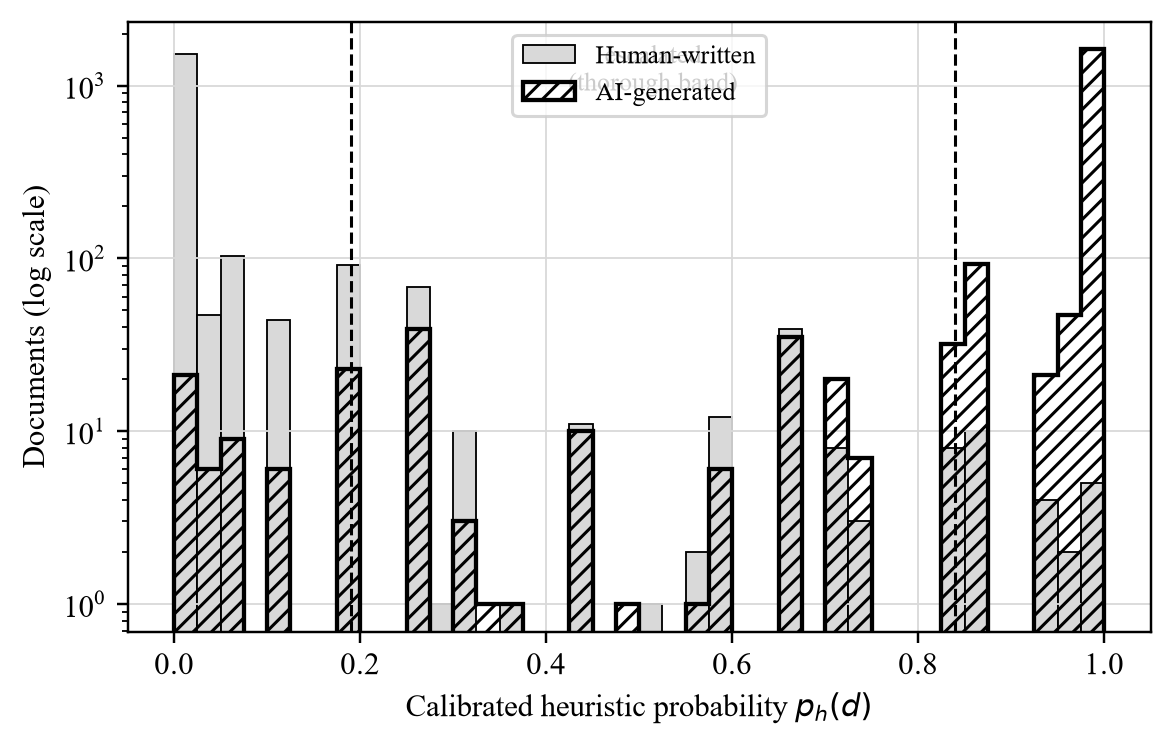
\includegraphics[width=0.84\textwidth]{ph_distribution.png}
\caption{Distribution of the calibrated heuristic probability on the test split, with the thorough band}
\label{fig:phdist}
\end{figure}

% ---------------------------------------------------------------------
\section{Result Analysis}
% ---------------------------------------------------------------------

\subsection{In-Distribution Accuracy}

Table~\ref{tab:testresults} gives the results on the test split (4,000
documents from the same sources, domains and generator families as the
training data, but from disjoint question groups).

\begin{table}[H]
\caption{Results on the in-distribution test split ($n = 4000$)}
\label{tab:testresults}
\centering
\footnotesize\setlength{\tabcolsep}{3pt}
\begin{tabularx}{\textwidth}{|p{2.9cm}|C|C|C|C|C|C|C|C|}
\hline
\textbf{System} & \textbf{Acc.} & \textbf{Prec.} & \textbf{Recall} & \textbf{F1} & \textbf{AUROC} & \textbf{FPR} & \textbf{ECE} & \textbf{Esc.} \\ \hline
Heuristic only & 0.9465 & 0.9524 & 0.9400 & 0.9461 & 0.9878 & 4.70\% & 0.015 & 0\% \\ \hline
Transformer only & 0.9740 & 0.9523 & \textbf{0.9980} & \textbf{0.9746} & \textbf{0.9992} & 5.00\% & 0.026 & 100\% \\ \hline
Cascade, fast & 0.9467 & 0.9524 & 0.9405 & 0.9464 & 0.9878 & 4.70\% & 0.015 & 0.0\% \\ \hline
Cascade, balanced & 0.9487 & 0.9517 & 0.9455 & 0.9486 & 0.9881 & 4.80\% & 0.015 & 0.6\% \\ \hline
Cascade, thorough & \textbf{0.9713} & \textbf{0.9753} & 0.9670 & 0.9711 & 0.9913 & \textbf{2.45\%} & 0.015 & 8.0\% \\ \hline
\end{tabularx}
\end{table}

The transformer is the most accurate single model (F1 0.9746, AUROC 0.9992),
and the heuristic is about 2.9 points of F1 behind it (0.9461). The thorough
cascade, which sends 8\% of the documents to the transformer, reaches F1 0.9711
and recovers 88\% of the gap. The paired bootstrap shows that the remaining
difference to the transformer is not significant
($\Delta F_1 = -0.0035$, 95\% CI $[-0.0095, +0.0023]$, $p = 0.24$), while the
improvement over the heuristic is (+0.025). The balanced cascade is
significantly worse than the transformer ($\Delta F_1 = -0.026$, CI
$[-0.034, -0.019]$) and only marginally better than the heuristic
($+0.0024$, CI $[+0.0007, +0.0043]$). Table~\ref{tab:bootstrap} lists the
confidence intervals.

\begin{table}[H]
\caption{95\% bootstrap confidence intervals on the test split (1000 resamples)}
\label{tab:bootstrap}
\centering
\small
\begin{adjustbox}{max width=\textwidth}\begin{tabular}{|l|c|c|}
\hline
\textbf{System} & \textbf{F1} & \textbf{AUROC} \\ \hline
Heuristic only & 0.9461 [0.9389, 0.9535] & 0.9878 [0.9849, 0.9904] \\ \hline
Transformer only & 0.9746 [0.9694, 0.9795] & 0.9992 [0.9987, 0.9995] \\ \hline
Cascade, balanced & 0.9486 [0.9416, 0.9559] & 0.9881 [0.9853, 0.9907] \\ \hline
Cascade, thorough & 0.9711 [0.9658, 0.9763] & 0.9913 [0.9886, 0.9936] \\ \hline
\end{tabular}\end{adjustbox}
\end{table}

The confusion matrices (Table~\ref{tab:confusion}) show \emph{how} the systems
differ. The transformer almost never misses an AI-generated text (4 false
negatives) but flags 100 of the 2,000 human texts. The heuristic makes a
similar number of false positives (94) and many more false negatives (120).
The thorough cascade has \textbf{the fewest false positives of all systems
(49)}, about half of either baseline, at the price of 66 false negatives.

\begin{table}[H]
\caption{Confusion matrices on the test split (2,000 human-written and 2,000 AI-generated documents)}
\label{tab:confusion}
\centering
\small
\begin{adjustbox}{max width=\textwidth}\begin{tabular}{|l|c|c|c|c|}
\hline
\textbf{System} & \textbf{TP} & \textbf{FN} & \textbf{FP} & \textbf{TN} \\ \hline
Heuristic only & 1880 & 120 & 94 & 1906 \\ \hline
Transformer only & 1996 & 4 & 100 & 1900 \\ \hline
Cascade, balanced & 1891 & 109 & 96 & 1904 \\ \hline
Cascade, thorough & 1934 & 66 & \textbf{49} & 1951 \\ \hline
\end{tabular}\end{adjustbox}
\end{table}

The reason is that the two stages make different mistakes. Of the 320 test
documents that the thorough gate escalates, the heuristic would have labelled
only 60.0\% correctly, whereas the transformer labels 90.9\% of them
correctly; on the 3,680 documents that stay on the fast path the heuristic is
97.7\% correct. The heuristic's confident decisions are therefore more
reliable than the transformer's on human texts, and the transformer is
reliable precisely where the heuristic is unsure. The ROC curves
(Fig.~\ref{fig:roc}) confirm the ranking by AUROC; the inset shows the region of
low false positive rate that matters in practice.

\begin{figure}[H]
\centering
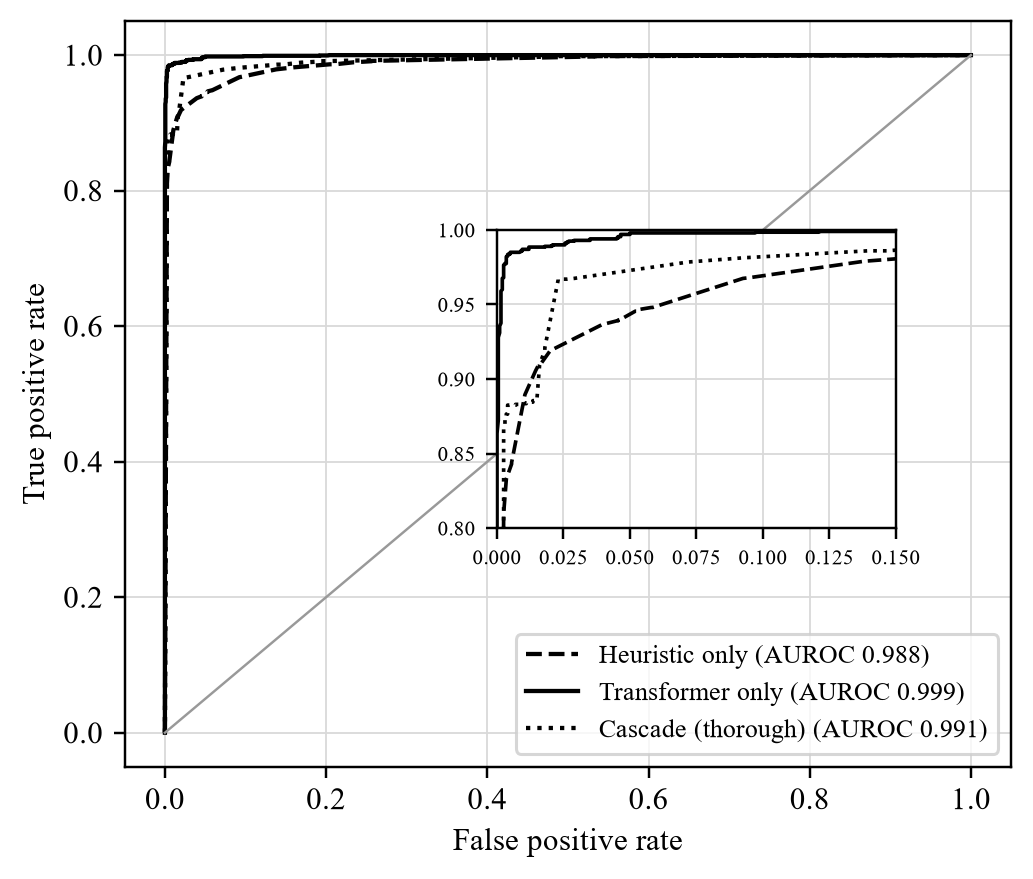
\includegraphics[width=0.66\textwidth]{roc_test.png}
\caption{ROC curves on the test split (inset: false positive rate below 15\%)}
\label{fig:roc}
\end{figure}

\subsection{Accuracy--Cost Trade-off}

Fig.~\ref{fig:tradeoffres} plots the operating points obtained by sweeping the
weight $\lambda$ of Eq.~\eqref{eq:lagrangian} on the validation split, with
the measured CPU costs of the two stages. Two observations stand out. First,
F1 rises steeply as the first few per cent of documents are escalated, and the
thorough point lies just below the knee of the curve. Second, cascades that
escalate between 20\% and 30\% of the documents \emph{exceed} the
transformer's own F1 on the validation split (0.987 against 0.983), which again
shows that the two stages are complementary rather than redundant. However,
the standalone transformer is the leftmost point at high accuracy: because the
heuristic stage is more expensive than the transformer (Section~\ref{sec:efficiency}),
every cascade costs more than running the transformer alone.

\begin{figure}[H]
\centering
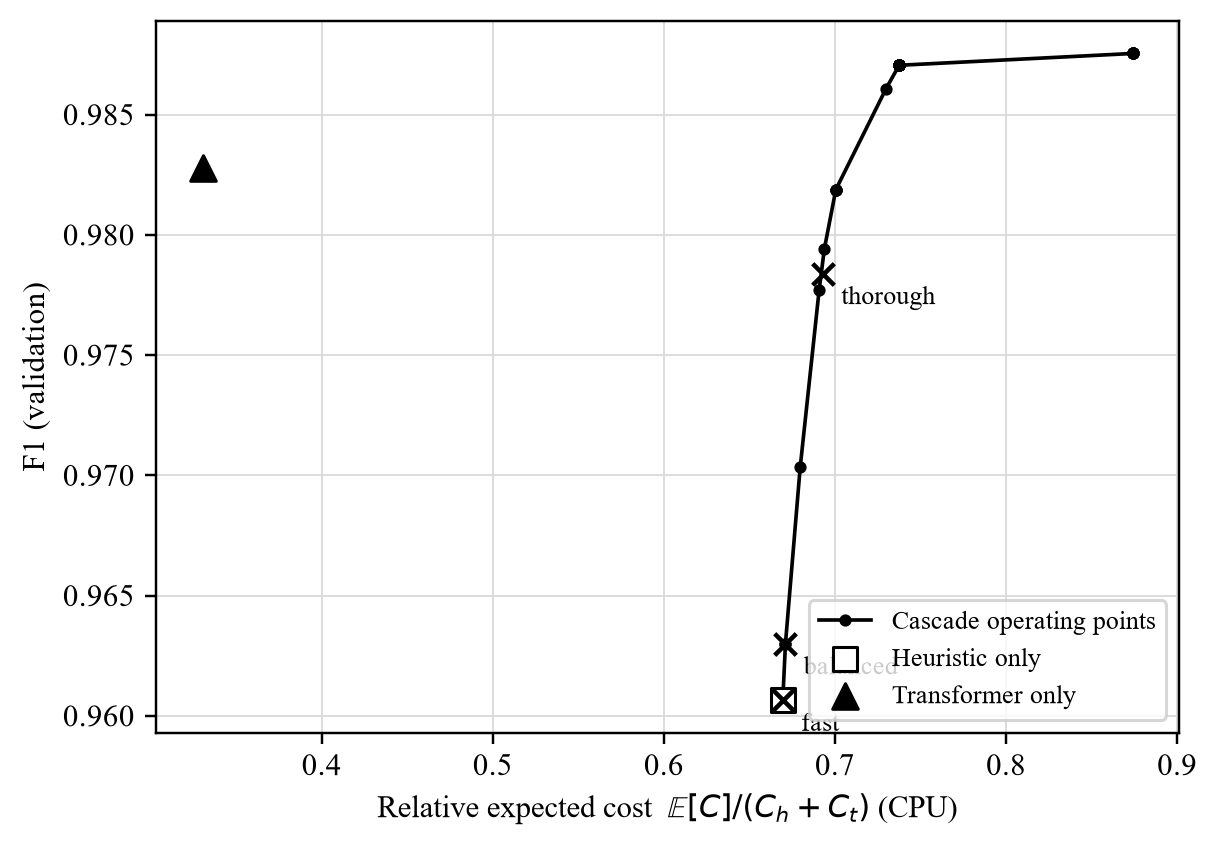
\includegraphics[width=0.78\textwidth]{tradeoff_val.png}
\caption{Accuracy--cost trade-off of the cascade on the validation split (measured CPU costs)}
\label{fig:tradeoffres}
\end{figure}

\subsection{Breakdown by Source, Domain, Length and Generator}

Table~\ref{tab:bysource} breaks the test results down by source benchmark. On
HC3 the heuristic is as good as the transformer and the cascade is better than
both (0.989). M4 and RAID, which contain more generator families and more
varied domains, are harder for the heuristic; there the cascade lies between
the two baselines, and on RAID it is the best of the three.

\begin{table}[H]
\caption{F1 on the test split by source benchmark}
\label{tab:bysource}
\centering
\small
\begin{adjustbox}{max width=\textwidth}\begin{tabular}{|l|c|c|c|c|}
\hline
\textbf{Source} & \textbf{Documents} & \textbf{Heuristic} & \textbf{Transformer} & \textbf{Cascade, thorough} \\ \hline
HC3 & 1,890 & 0.9782 & 0.9783 & \textbf{0.9885} \\ \hline
M4 & 1,482 & 0.9212 & \textbf{0.9834} & 0.9570 \\ \hline
RAID & 628 & 0.9042 & 0.9440 & \textbf{0.9509} \\ \hline
\end{tabular}\end{adjustbox}
\end{table}

Table~\ref{tab:bylength} shows that accuracy depends little on length within the
range of the corpus (100 to 1,500 words). Documents above 500 words are
slightly easier for every system, and the escalation rate is somewhat higher
for medium-length documents.

\begin{table}[H]
\caption{F1 on the test split by document length}
\label{tab:bylength}
\centering
\small
\begin{adjustbox}{max width=\textwidth}\begin{tabular}{|l|c|c|c|c|c|}
\hline
\textbf{Length (words)} & \textbf{Documents} & \textbf{Heuristic} & \textbf{Transformer} & \textbf{Cascade, thorough} & \textbf{Escalated} \\ \hline
100--250 & 2,668 & 0.9453 & 0.9740 & 0.9698 & 7.2\% \\ \hline
250--500 & 995 & 0.9405 & 0.9728 & 0.9710 & 9.8\% \\ \hline
over 500 & 337 & 0.9699 & 0.9853 & 0.9820 & 8.9\% \\ \hline
\end{tabular}\end{adjustbox}
\end{table}

Because the human texts are shared between generator families and domains,
the per-family and per-domain results are reported as the detection rate
(recall) on the AI texts of that family or domain
(Tables~\ref{tab:byfamily} and~\ref{tab:bydomain}). The heuristic detects
ChatGPT-style text very reliably (97\%) but misses one in five Dolly texts
and one in nine Llama texts; the thorough cascade closes part of each gap. In
the domain breakdown the heuristic is weakest on arXiv abstracts (81\%),
news (86\%), poetry (86\%) and WikiHow articles (87\%), i.e.\ on formal or
formulaic human genres whose statistics resemble model output.

\begin{table}[H]
\caption{Detection rate (recall) on the test split by generator family}
\label{tab:byfamily}
\centering
\small
\begin{adjustbox}{max width=\textwidth}\begin{tabular}{|l|c|c|c|c|c|}
\hline
\textbf{Family} & \textbf{AI documents} & \textbf{Heuristic} & \textbf{Transformer} & \textbf{Cascade, balanced} & \textbf{Cascade, thorough} \\ \hline
GPT & 1,195 & 0.972 & 0.998 & 0.973 & 0.982 \\ \hline
Cohere & 248 & 0.919 & 1.000 & 0.935 & 0.964 \\ \hline
Dolly & 218 & 0.807 & 1.000 & 0.821 & 0.899 \\ \hline
BLOOMZ & 122 & 0.943 & 1.000 & 0.951 & 0.992 \\ \hline
Llama & 89 & 0.888 & 1.000 & 0.888 & 0.910 \\ \hline
MPT & 87 & 0.920 & 0.977 & 0.931 & 0.943 \\ \hline
Flan-T5 & 41 & 1.000 & 1.000 & 1.000 & 1.000 \\ \hline
\end{tabular}\end{adjustbox}
\end{table}

\begin{table}[H]
\caption{Detection rate (recall) on the test split by domain (domains with at least 50 AI documents)}
\label{tab:bydomain}
\centering
\small
\begin{adjustbox}{max width=\textwidth}\begin{tabular}{|l|c|c|c|c|}
\hline
\textbf{Domain (source)} & \textbf{AI documents} & \textbf{Heuristic} & \textbf{Transformer} & \textbf{Cascade, thorough} \\ \hline
Reddit ELI5 (HC3) & 781 & 0.996 & 1.000 & 0.999 \\ \hline
arXiv (M4) & 185 & 0.811 & 0.995 & 0.876 \\ \hline
Wikipedia (M4) & 175 & 0.926 & 1.000 & 0.977 \\ \hline
Reddit (M4) & 155 & 0.910 & 1.000 & 0.961 \\ \hline
WikiHow (M4) & 133 & 0.872 & 0.992 & 0.910 \\ \hline
Finance (HC3) & 119 & 1.000 & 1.000 & 1.000 \\ \hline
Abstracts (RAID) & 104 & 0.904 & 0.990 & 0.962 \\ \hline
PeerRead (M4) & 93 & 0.925 & 1.000 & 0.935 \\ \hline
News (RAID) & 77 & 0.857 & 1.000 & 0.948 \\ \hline
Books (RAID) & 75 & 0.973 & 0.987 & 0.987 \\ \hline
Poetry (RAID) & 58 & 0.862 & 1.000 & 0.914 \\ \hline
\end{tabular}\end{adjustbox}
\end{table}

\subsection{Calibration}

Fig.~\ref{fig:calib} is the reliability diagram on the test split. After
isotonic calibration the heuristic's probabilities follow the diagonal closely
(ECE 0.015), whereas the transformer is markedly over-confident: almost all of
its outputs are close to 0 or 1, and its ECE is 0.026 in distribution and rises
to 0.35 on MAGE (Table~\ref{tab:robust}). This matters for the gate, which
compares $p_h(d)$ with fixed thresholds: a threshold of 0.84 on the calibrated
heuristic means that about 84\% of documents scored there are AI-generated,
which is not true of the transformer's scores.

\begin{figure}[H]
\centering
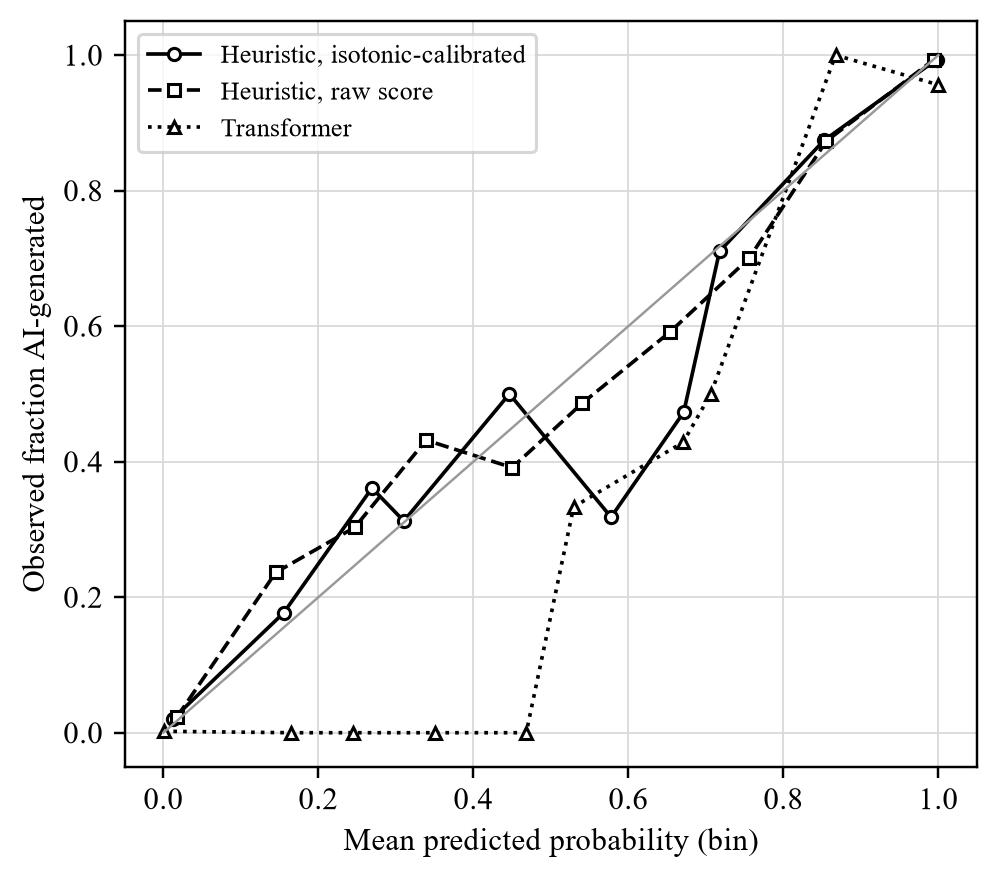
\includegraphics[width=0.62\textwidth]{calibration_test.png}
\caption{Reliability diagram on the test split}
\label{fig:calib}
\end{figure}

\textbf{Calibration ablation (RQ2).} To test whether calibration improves the
cascade's operating points, the band search was repeated with the uncalibrated
probability $\sigma(s_h(d))$ in place of $p_h(d)$, and the best validation F1
reachable at each escalation budget was compared (Table~\ref{tab:calabl}). The
two variants are within 0.003 of each other at every budget, and the raw score
is marginally ahead. Because isotonic calibration is monotonic, it changes the
values of the thresholds but not the order of the documents, so with a free
choice of band both variants can select the same set of documents. Calibration
therefore did not improve accuracy here; its value is that the thresholds,
the escalation rate and the reported probability have a direct
interpretation.

\begin{table}[H]
\caption{Best validation F1 of the cascade at a given escalation budget: calibrated vs.\ raw heuristic score}
\label{tab:calabl}
\centering
\small
\begin{adjustbox}{max width=\textwidth}\begin{tabular}{|c|c|c|}
\hline
\textbf{Maximum escalation rate} & \textbf{Calibrated $p_h$} & \textbf{Raw score $\sigma(s_h)$} \\ \hline
5\% & 0.9724 & 0.9751 \\ \hline
10\% & 0.9819 & 0.9821 \\ \hline
20\% & 0.9863 & 0.9873 \\ \hline
30\% & 0.9871 & 0.9878 \\ \hline
50\% & 0.9871 & 0.9879 \\ \hline
\end{tabular}\end{adjustbox}
\end{table}

\subsection{Generalisation to Unseen Generators}

\textbf{Held-out family (Mistral).} The Mistral family was removed from every
step of training, calibration and tuning. Table~\ref{tab:heldout} shows that
all systems lose accuracy on it. The transformer loses least
(0.9746 $\rightarrow$ 0.9576), the heuristic most (0.9461 $\rightarrow$ 0.9065),
and the thorough cascade lies between them (0.9711 $\rightarrow$ 0.9285); its
difference from the transformer is now significant ($-0.029$, CI
$[-0.049, -0.010]$). The escalation rate of the thorough cascade rises from
8.0\% to 10.1\%, so the gate does send more of the unfamiliar documents to the
second stage, but not enough of them: the heuristic misses 14\% of the Mistral
texts, and many of these misses are confident.

\begin{table}[H]
\caption{Results on the held-out generator family (Mistral, 372 AI + 372 human documents)}
\label{tab:heldout}
\centering
\small
\begin{tabularx}{\textwidth}{|p{2.9cm}|C|C|C|C|C|C|}
\hline
\textbf{System} & \textbf{Prec.} & \textbf{Recall} & \textbf{F1 [95\% CI]} & \textbf{AUROC} & \textbf{FPR} & \textbf{Esc.} \\ \hline
Heuristic only & 0.958 & 0.860 & 0.907 [0.882, 0.928] & 0.964 & 3.8\% & 0\% \\ \hline
Transformer only & 0.945 & \textbf{0.970} & \textbf{0.958} [0.943, 0.972] & \textbf{0.995} & 5.7\% & 100\% \\ \hline
Cascade, balanced & 0.956 & 0.874 & 0.913 [0.890, 0.934] & 0.965 & 4.0\% & 1.3\% \\ \hline
Cascade, thorough & \textbf{0.971} & 0.890 & 0.929 [0.908, 0.947] & 0.965 & \textbf{2.7\%} & 10.1\% \\ \hline
\end{tabularx}
\end{table}

\textbf{Leave-one-generator-out for the heuristic stage.} The heuristic stage
was retrained seven more times, each time without one of the remaining
families, and evaluated on that family's AI texts in the test split
(Fig.~\ref{fig:logo}, Table~\ref{tab:logo}). For four of the seven families
(GPT, Cohere, MPT and Flan-T5) the detection rate falls by less than six
points: the statistical signature learned from the other families transfers.
Dolly and Llama lose eight to nine points. BLOOMZ is the clear exception: its
detection rate collapses from 0.943 to 0.320 when it is not in the training
data. BLOOMZ was instruction-tuned on a task mixture that differs from that of
the other models, and its texts evidently do not share their statistical
profile, so a detector must have seen examples of it.

\begin{figure}[H]
\centering
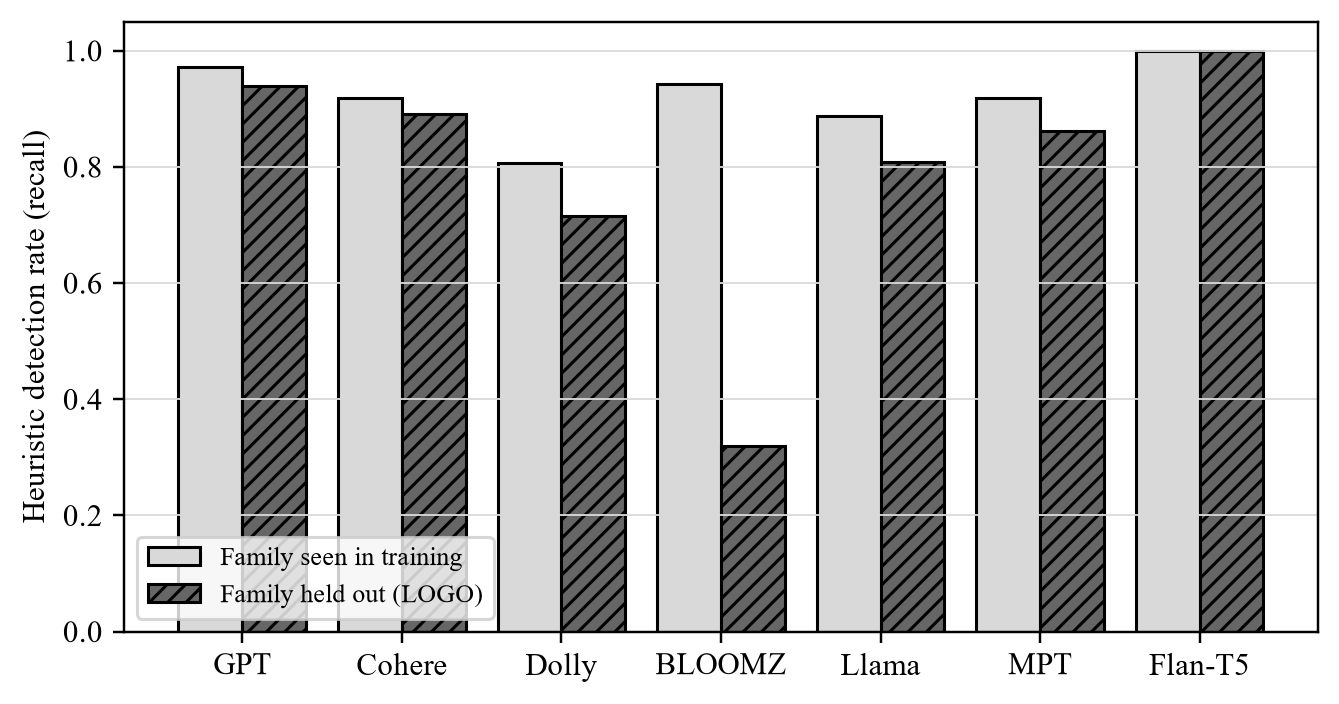
\includegraphics[width=0.84\textwidth]{logo_recall.png}
\caption{Heuristic detection rate per generator family, with the family in and out of the training data}
\label{fig:logo}
\end{figure}

\begin{table}[H]
\caption{Leave-one-generator-out results for the heuristic stage (test split)}
\label{tab:logo}
\centering
\small
\begin{adjustbox}{max width=\textwidth}\begin{tabular}{|l|c|c|c|c|}
\hline
\textbf{Held-out family} & \textbf{AI documents} & \textbf{Recall, family seen} & \textbf{Recall, family held out} & \textbf{Change} \\ \hline
GPT & 1,195 & 0.972 & 0.940 & $-0.032$ \\ \hline
Cohere & 248 & 0.919 & 0.891 & $-0.028$ \\ \hline
Dolly & 218 & 0.807 & 0.716 & $-0.092$ \\ \hline
BLOOMZ & 122 & 0.943 & 0.320 & $-0.623$ \\ \hline
Llama & 89 & 0.888 & 0.809 & $-0.079$ \\ \hline
MPT & 87 & 0.920 & 0.862 & $-0.057$ \\ \hline
Flan-T5 & 41 & 1.000 & 1.000 & $0.000$ \\ \hline
\end{tabular}\end{adjustbox}
\end{table}

\textbf{Full-cascade leave-one-out (Llama).} For the Llama family, a second
RoBERTa model was also trained without Llama, so the complete cascade can be
evaluated on a family that neither stage has seen (Table~\ref{tab:llamalogo}).
The transformer still detects every Llama text, and the cascade's detection
rate falls less than the heuristic's (0.910 $\rightarrow$ 0.876). On the 2,000
human test texts, the models trained without Llama produce fewer false
positives, and the cascade again has the lowest false positive rate (2.0\%).
For Llama, escalation is 14.6\% with and without the family in training, well
above the 8\% average, so Llama texts are disproportionately routed to the
transformer whether or not they were seen.

\begin{table}[H]
\caption{Full-cascade leave-one-generator-out for Llama (89 Llama texts, 2,000 human texts of the test split)}
\label{tab:llamalogo}
\centering
\small
\begin{adjustbox}{max width=\textwidth}\begin{tabular}{|l|c|c|c|c|}
\hline
 & \multicolumn{2}{c|}{\textbf{Llama in training}} & \multicolumn{2}{c|}{\textbf{Llama held out}} \\ \cline{2-5}
\textbf{System} & \textbf{Recall (Llama)} & \textbf{FPR (humans)} & \textbf{Recall (Llama)} & \textbf{FPR (humans)} \\ \hline
Heuristic only & 0.888 & 4.70\% & 0.809 & 3.35\% \\ \hline
Transformer only & 1.000 & 5.00\% & 1.000 & 3.85\% \\ \hline
Cascade, thorough & 0.910 & \textbf{2.45\%} & 0.876 & \textbf{2.00\%} \\ \hline
\end{tabular}\end{adjustbox}
\end{table}

\subsection{Robustness: Out-of-Distribution Data and Attacks}

Table~\ref{tab:robust} and Fig.~\ref{fig:splitf1} compare the systems on the
three test sets that come from outside the training distribution. The picture
changes sharply.

\begin{table}[H]
\caption{Results on out-of-distribution and adversarial test sets}
\label{tab:robust}
\centering
\small
\begin{tabularx}{\textwidth}{|p{2.6cm}|p{2.6cm}|C|C|C|C|C|}
\hline
\textbf{Test set} & \textbf{System} & \textbf{Recall} & \textbf{FPR} & \textbf{F1} & \textbf{ECE} & \textbf{Esc.} \\ \hline
\multirow{3}{*}{\makecell[l]{MAGE OOD\\(1,433 docs)}} & Heuristic & 0.913 & \textbf{20.5\%} & \textbf{0.857} & 0.074 & 0\% \\ \cline{2-7}
 & Transformer & 1.000 & 69.3\% & 0.732 & 0.351 & 100\% \\ \cline{2-7}
 & Cascade, thorough & 0.954 & 30.6\% & 0.838 & 0.152 & 22.0\% \\ \hline
\multirow{3}{*}{\makecell[l]{MAGE OOD\\paraphrased\\(1,500 docs)}} & Heuristic & 0.519 & \textbf{17.7\%} & 0.607 & 0.156 & 0\% \\ \cline{2-7}
 & Transformer & 0.996 & 92.3\% & 0.666 & 0.472 & 100\% \\ \cline{2-7}
 & Cascade, thorough & 0.747 & 37.3\% & \textbf{0.695} & 0.273 & 43.7\% \\ \hline
\multirow{3}{*}{\makecell[l]{RAID attacks\\(690 AI docs)}} & Heuristic & 0.844 & -- & 0.915 & 0.185 & 0\% \\ \cline{2-7}
 & Transformer & \textbf{0.987} & -- & \textbf{0.993} & 0.014 & 100\% \\ \cline{2-7}
 & Cascade, thorough & 0.913 & -- & 0.955 & 0.095 & 21.4\% \\ \hline
\end{tabularx}
\end{table}

\begin{figure}[H]
\centering
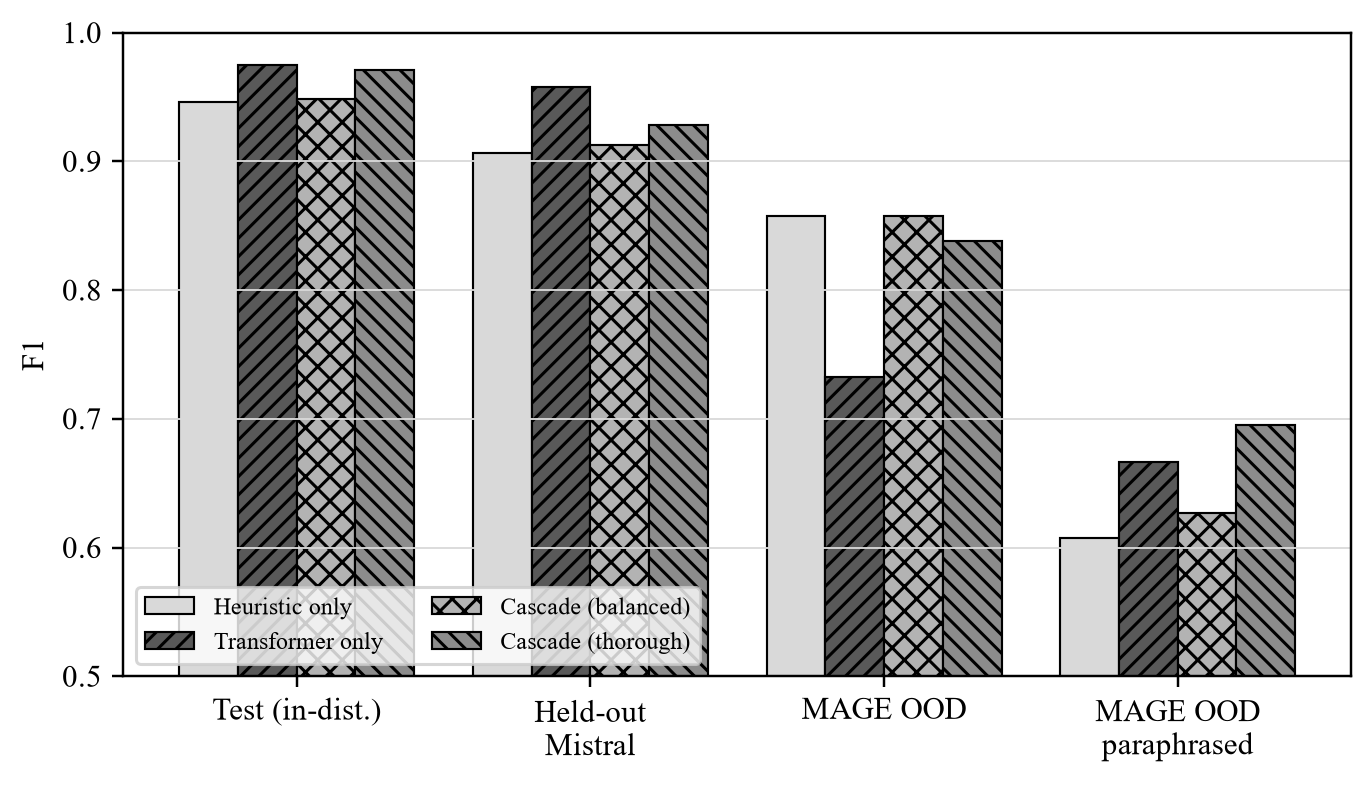
\includegraphics[width=0.92\textwidth]{f1_by_split.png}
\caption{F1 of the four main systems on the in-distribution, held-out-generator and out-of-distribution test sets}
\label{fig:splitf1}
\end{figure}

\textbf{MAGE out-of-distribution.} On texts from domains that are absent from
the training data, the fine-tuned transformer labels almost everything as
AI-generated: it flags 69\% of the human texts, and 92\% after paraphrasing.
It has learned cues that are specific to the training domains rather than to
machine authorship. The heuristic, whose features describe generic statistical
properties of text, degrades far more gracefully (FPR 20.5\%, F1 0.857). The
cascade inherits part of the transformer's failure through the documents it
escalates, and its F1 (0.838) is significantly better than the transformer's
($+0.106$, CI $[+0.089, +0.124]$) but slightly below the heuristic's. On the
paraphrased set, paraphrasing pushes most AI texts into the human range of the
heuristic features (recall 0.52), and the cascade, which escalates 44\% of these
texts, is the best of the three systems (F1 0.695). In both MAGE sets the
escalation rate rises sharply (from 8\% to 22\% and 44\%), which shows that the
gate recognises that these documents are unusual.

\textbf{RAID attacks.} The eleven RAID attacks are character- and word-level
perturbations of AI texts. The transformer is almost unaffected (98.7\%
detected), whereas the heuristic's detection rate falls to 84\%
(Fig.~\ref{fig:raid}). Synonym substitution (67\%), upper/lower-case changes
(73\%) and paraphrasing (73\%) hurt the heuristic most, because they change
token probabilities directly; zero-width spaces and inserted paragraphs barely
affect it. Escalation rises to 21\% on attacked texts and the thorough cascade
recovers about half of the heuristic's loss (91.3\% detected).

\begin{figure}[H]
\centering
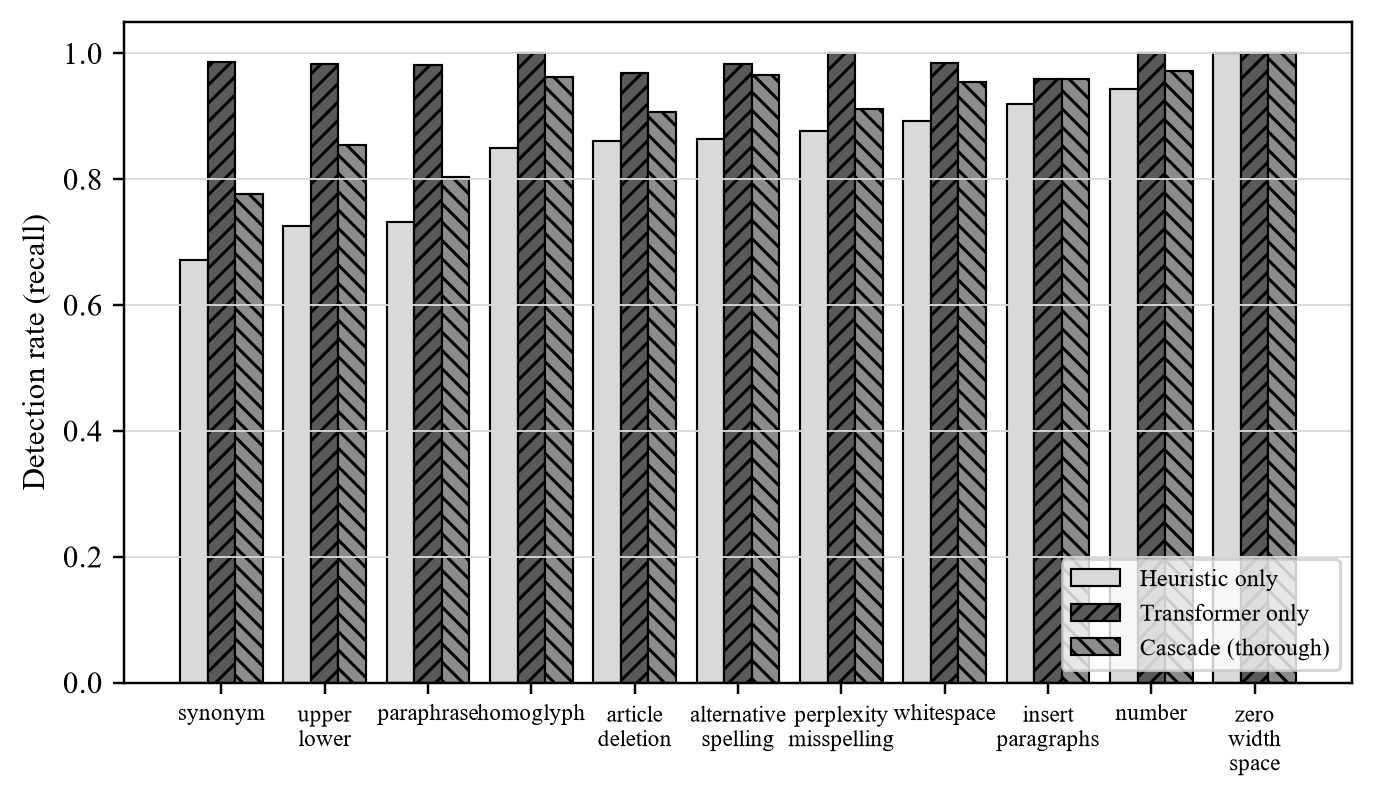
\includegraphics[width=0.92\textwidth]{raid_attacks.png}
\caption{Detection rate on the RAID adversarial attacks}
\label{fig:raid}
\end{figure}

\subsection{Fairness to Non-Native Writers}
\label{sec:fairnessres}

Table~\ref{tab:fairness} and Fig.~\ref{fig:fairness} report the false positive
rates on the fairness test set: 81 essays by native speakers and 47 TOEFL essays
by non-native speakers, all human-written.

\begin{table}[H]
\caption{False positive rates on human-written essays (fairness test set)}
\label{tab:fairness}
\centering
\small
\begin{adjustbox}{max width=\textwidth}\begin{tabular}{|l|c|c|c|}
\hline
\textbf{System} & \textbf{FPR native (81)} & \textbf{FPR non-native (47)} & $\Delta_{FPR}$ \\ \hline
Heuristic only & \textbf{2.5\%} & \textbf{17.0\%} & 0.146 \\ \hline
Transformer only & 51.9\% & 63.8\% & \textbf{0.120} \\ \hline
Cascade, fast / balanced & \textbf{2.5\%} & \textbf{17.0\%} & 0.146 \\ \hline
Cascade, thorough & \textbf{2.5\%} & 25.5\% & 0.231 \\ \hline
\end{tabular}\end{adjustbox}
\end{table}

\begin{figure}[H]
\centering
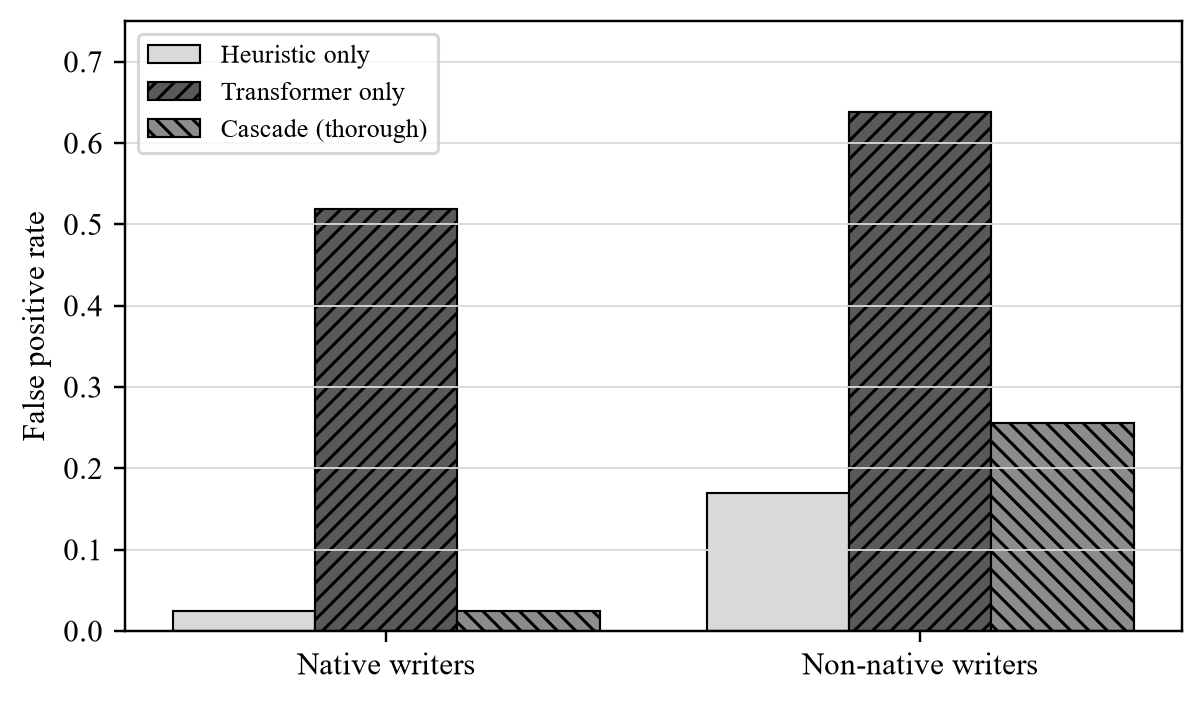
\includegraphics[width=0.74\textwidth]{fairness_fpr.png}
\caption{False positive rates on native and non-native human-written essays}
\label{fig:fairness}
\end{figure}

Three findings follow. First, \textbf{all systems flag non-native writing more
often than native writing}, confirming the bias reported by Liang
\textit{et al.}~\cite{liang2023biased}. Second, \textbf{the transformer is by
far the least fair system in absolute terms}: it flags more than half of the
native student essays and nearly two thirds of the non-native ones. Like the
MAGE result, this is a failure of the fine-tuned model on a genre (school and
admission essays) that is not in its training data. Third, the transformer has
the \emph{smallest disparity}, but only because it is almost equally wrong for
both groups.

This third finding is why the worst-group form of the fairness constraint was
adopted. With the disparity form ($\Delta_{FPR}$ no larger than the transformer's
plus one standard error), the band search for the thorough point returned
$[0.00, 0.84]$: it escalates every essay with $p_h \le 0.84$, i.e.\ 54\% of all
validation documents, and reaches the required disparity by raising the
native writers' false positive rate from 3.9\% to 50.6\% on the fairness
validation set. A constraint that is satisfied by harming one group without
helping the other is not a meaningful fairness guarantee. The worst-group
constraint (non-native FPR no higher than the transformer's) cannot be gamed in
this way and yields the band $[0.19, 0.84]$ with 7.1\% escalation; with this
band the cascade flags 2.5\% of native and 25.5\% of non-native essays on the
test set. This is higher for non-native writers than the heuristic alone
(17.0\%), because the essays that the gate escalates are sent to the biased
transformer, but it is far below the transformer's 63.8\%. The fairness sets are
small (one non-native essay is 2.1 percentage points), so these differences
carry considerable uncertainty.

\subsection{Efficiency}
\label{sec:efficiency}

Table~\ref{tab:latency} and Fig.~\ref{fig:latency} report the latency measured
with the protocol of Section~6.1.5 on 200 test documents.

\begin{table}[H]
\caption{Latency and throughput (200 test documents after 20 warm-up documents)}
\label{tab:latency}
\centering
\small
\begin{tabularx}{\textwidth}{|p{1.3cm}|p{2.7cm}|C|C|C|C|C|}
\hline
\textbf{Device} & \textbf{System} & \textbf{Mean (ms)} & \textbf{p95 (ms)} & \textbf{Docs/s} & \textbf{Docs/s, batch 32} & \textbf{Esc.} \\ \hline
\multirow{5}{*}{CPU} & Heuristic only & 353.9 & 788.1 & 2.83 & 2.9 & 0\% \\ \cline{2-7}
 & Transformer only & \textbf{174.7} & \textbf{477.3} & \textbf{5.72} & \textbf{5.4} & 100\% \\ \cline{2-7}
 & Cascade, fast & 358.8 & 828.7 & 2.79 & 2.8 & 0\% \\ \cline{2-7}
 & Cascade, balanced & 360.0 & 821.9 & 2.78 & 2.9 & 0\% \\ \cline{2-7}
 & Cascade, thorough & 362.5 & 759.1 & 2.76 & 2.7 & 7\% \\ \hline
\multirow{5}{*}{GPU} & Heuristic only & 73.0 & 133.0 & 13.7 & 14.1 & 0\% \\ \cline{2-7}
 & Transformer only & \textbf{10.0} & \textbf{14.3} & \textbf{100.5} & \textbf{252.3} & 100\% \\ \cline{2-7}
 & Cascade, fast & 71.8 & 128.7 & 13.9 & 13.7 & 0\% \\ \cline{2-7}
 & Cascade, balanced & 72.6 & 140.0 & 13.8 & 14.0 & 0\% \\ \cline{2-7}
 & Cascade, thorough & 73.6 & 134.5 & 13.6 & 13.9 & 7\% \\ \hline
\end{tabularx}
\end{table}

\begin{figure}[H]
\centering
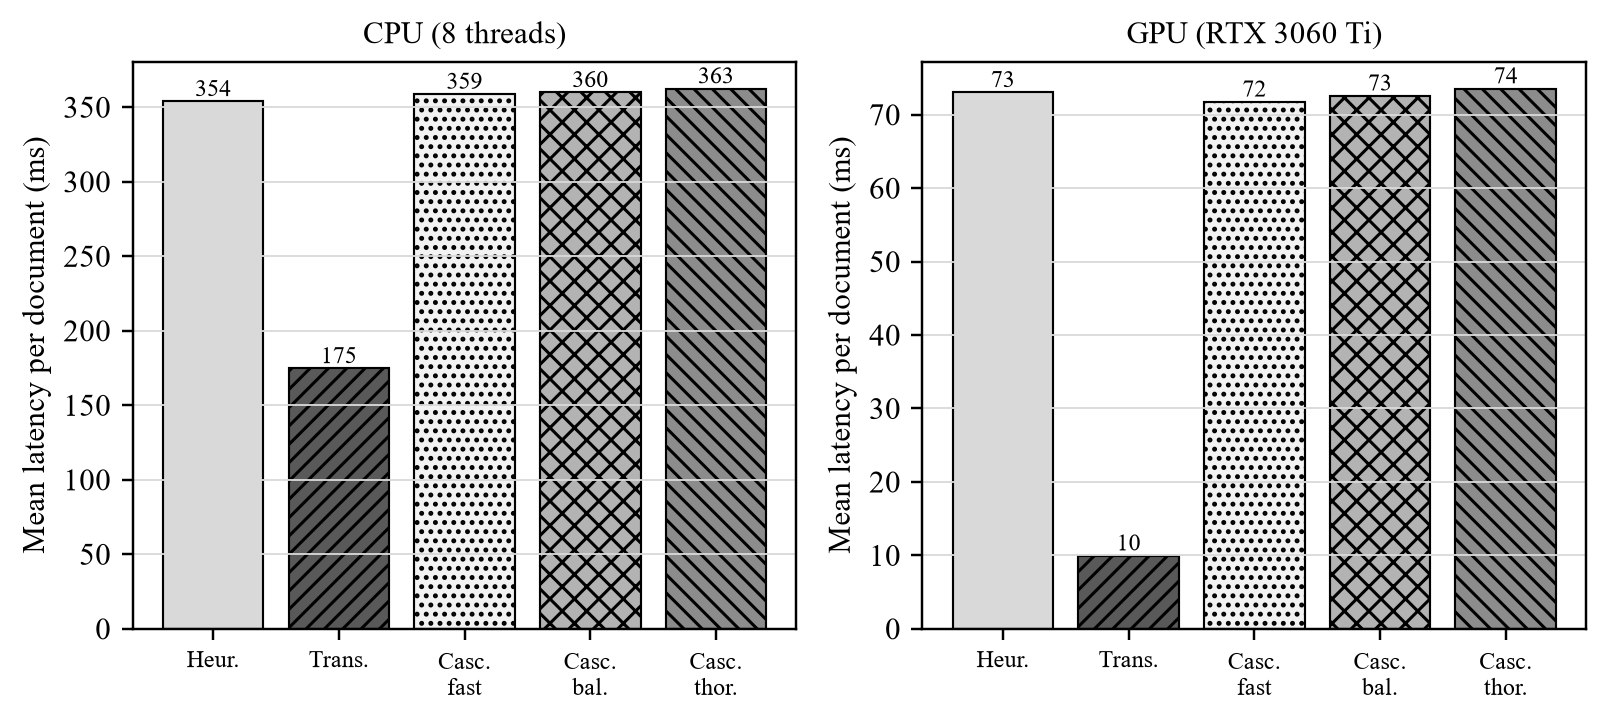
\includegraphics[width=0.94\textwidth]{latency.png}
\caption{Mean latency per document on CPU and GPU}
\label{fig:latency}
\end{figure}

\textbf{The cascade is slower than the transformer alone}, by a factor of 2.1
on the CPU and 7.4 on the GPU. The premise of Eq.~\eqref{eq:cascadecost},
$C_t \gg C_h$, does not hold for the implemented stages, and the measured
latencies agree with the decomposition
$\bar{t}_{\text{cascade}} \approx \bar{t}_h + \hat{\alpha}\,\bar{t}_t$
(on CPU: $353.9 + 0.07 \times 174.7 \approx 366$~ms against 362.5~ms measured).
Profiling the heuristic stage (Table~\ref{tab:profile}) shows where the time
goes.

\begin{table}[H]
\caption{Cost of the components of the heuristic stage per document}
\label{tab:profile}
\centering
\small
\begin{adjustbox}{max width=\textwidth}\begin{tabular}{|l|c|c|}
\hline
\textbf{Component} & \textbf{CPU (ms)} & \textbf{GPU (ms)} \\ \hline
spaCy sentence segmentation and POS tagging & 29 & 24 (runs on the CPU) \\ \hline
GPT-2 pass and token statistics (up to 2,048 tokens) & 316 & 15 \\ \hline
\quad of which: transformer body & 150 & -- \\ \hline
\quad of which: projection onto the 50,257-token vocabulary & 91 & -- \\ \hline
\quad of which: log-softmax, ranks and entropies & 30 & -- \\ \hline
Stylometric features, XGBoost head, calibration, explanation & $<$ 10 & $<$ 35 \\ \hline
\textbf{RoBERTa-base classification (for comparison)} & \textbf{175} & \textbf{10} \\ \hline
\end{tabular}\end{adjustbox}
\end{table}

On the CPU, the GPT-2 reference model is the bottleneck. GPT-2 small has the
same number of parameters as RoBERTa-base (124 million) and the same depth, so
its body alone costs about as much as the whole RoBERTa classification; on top
of that, a language model must project every token onto its 50,257-word
vocabulary and the heuristic statistics then scan this matrix several times,
which a classifier does not need to do. In addition, the reference model
reads up to 2,048 tokens of a document whereas the classifier reads one
512-token window for 87\% of the documents. On the GPU both networks are fast
and the CPU-bound parts of the heuristic stage dominate: spaCy alone takes
2.4 times as long as the entire RoBERTa classification, and the
per-document XGBoost explanation adds further overhead. Batching helps the
transformer (252 documents per second with batches of 32 on the GPU) but not the
heuristic stage, whose spaCy and per-document feature computation are
sequential.

The figures of merit of Eq.~\eqref{eq:recovery} summarise the outcome
(Table~\ref{tab:fom}). The thorough cascade recovers 88\% of the transformer's
accuracy advantage, but at a speed-up of 0.48 on the CPU and 0.14 on the GPU,
i.e.\ it is slower, not faster. The model footprint points the same way: the
heuristic stage needs the 548~MB GPT-2 model in addition to its 1.6~MB head,
which is more than the 480~MB RoBERTa classifier.

\begin{table}[H]
\caption{Figures of merit of the cascade (test split, Eq.~\eqref{eq:recovery})}
\label{tab:fom}
\centering
\small
\begin{adjustbox}{max width=\textwidth}\begin{tabular}{|l|c|c|c|}
\hline
\textbf{Operating point} & \textbf{Recovery} & \textbf{Speed-up (CPU)} & \textbf{Speed-up (GPU)} \\ \hline
Fast & 0.01 & 0.49 & 0.14 \\ \hline
Balanced & 0.09 & 0.49 & 0.14 \\ \hline
Thorough & 0.88 & 0.48 & 0.14 \\ \hline
\end{tabular}\end{adjustbox}
\end{table}

\subsection{Explainability}

Every fast-path decision is returned with its five most influential features,
their values and the median values of human-written and AI-generated training
documents (Listing~\ref{lst:json}, Fig.~\ref{fig:webui}); every escalated
decision states that the transformer decided and reports both probabilities.
Fig.~\ref{fig:importance} shows which features the XGBoost head relies on
overall. The perplexity group dominates: mean token log-probability and document
perplexity together account for 56\% of the total split gain, followed by the
type-token ratio (6\%), the mean predictive entropy (5\%) and the spread of
token log-probabilities (4\%). Burstiness, function-word rate, word length,
GLTR rank fractions, punctuation and POS bigrams each contribute between 1\%
and 3\%. This agrees with the literature reviewed in Chapter~\ref{ch:lit}:
token probability under a reference model is the strongest single signal, and
stylometric features add smaller, complementary evidence.

\begin{figure}[H]
\centering
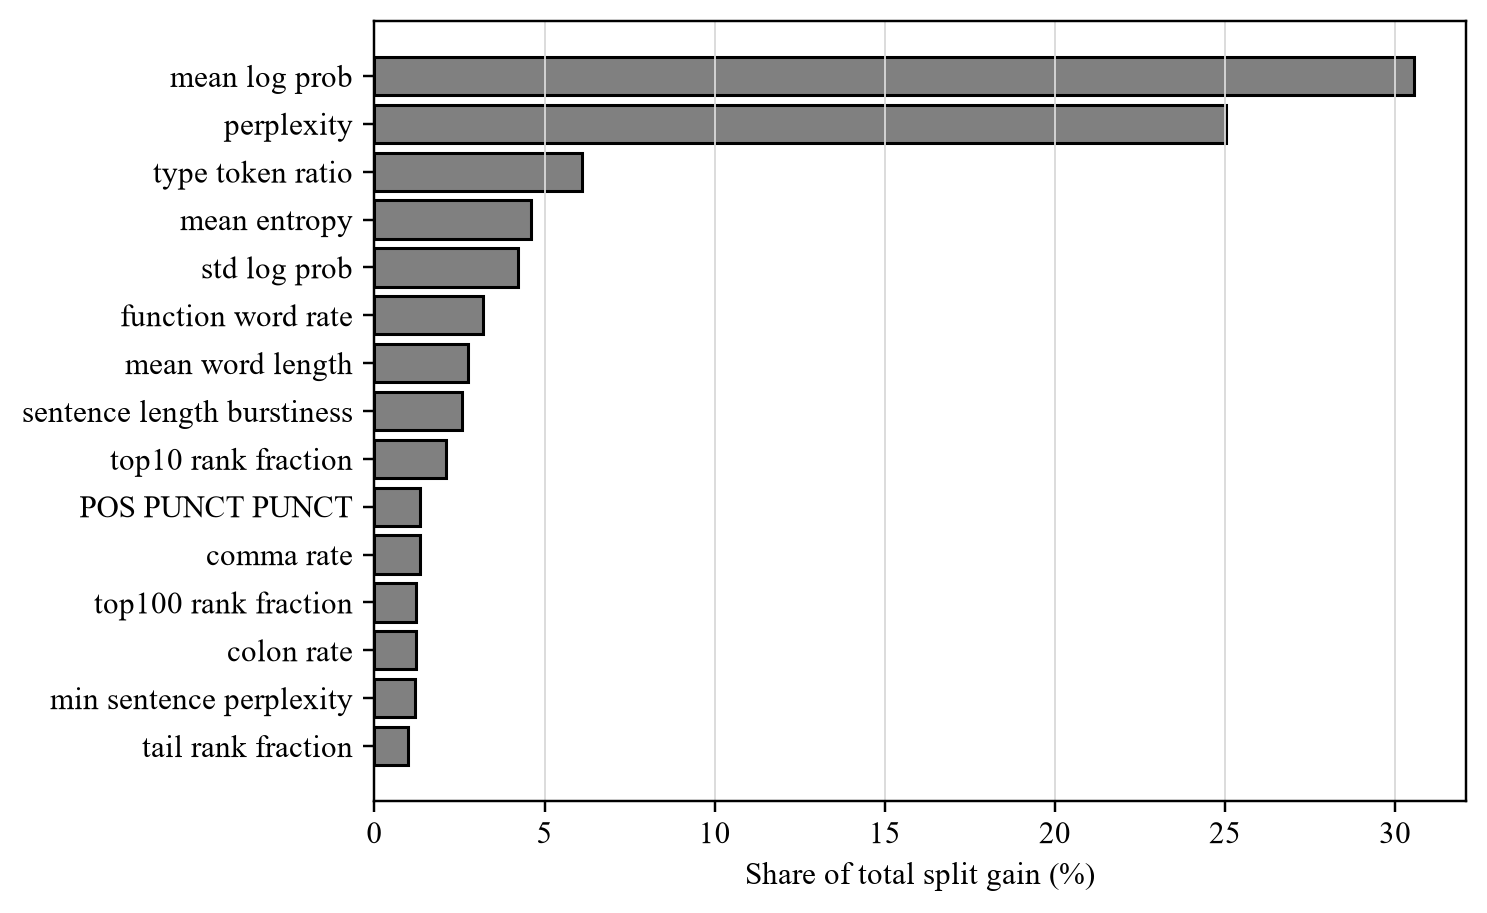
\includegraphics[width=0.78\textwidth]{feature_importance.png}
\caption{Fifteen most important features of the XGBoost heuristic head (share of total split gain)}
\label{fig:importance}
\end{figure}

% ---------------------------------------------------------------------
\section{Assessment Against the Success Criteria}
% ---------------------------------------------------------------------

Table~\ref{tab:criteria-status} compares the results with the success criteria
that were fixed in Table~\ref{tab:gap-obj} before the experiments.

\begin{table}[H]
\caption{Status of the success criteria of Table~\ref{tab:gap-obj}}
\label{tab:criteria-status}
\centering
\small
\begin{tabularx}{\textwidth}{|p{2.5cm}|p{4.0cm}|L|p{1.5cm}|}
\hline
\textbf{Problem} & \textbf{Criterion} & \textbf{Result} & \textbf{Status} \\ \hline
P1 Black box & Every fast-path decision reported with its top features & Implemented in the library, CLI, API and web page; five features with human and AI medians per decision & Met \\ \hline
P2 Cost and licensing & Runs locally on open-source software, no per-document charge & All components open source; all experiments run on one workstation; no document leaves the machine & Met \\ \hline
P3 Latency at scale & Cascade mean latency $\ge$ 50\% below transformer-only on CPU & 362.5 ms against 174.7 ms: 2.1 times \emph{slower} (Table~\ref{tab:latency}) & Not met \\ \hline
P4 Generator overfitting & Cascade F1 on a held-out generator reported and compared & Mistral: 0.929 vs.\ 0.958 (transformer) and 0.907 (heuristic); LOGO for 7 families and full-cascade LOGO for Llama & Met \\ \hline
P5 Fairness & $\Delta_{FPR}$ of cascade $\le$ that of transformer-only & 0.231 (thorough) and 0.146 (balanced) vs.\ 0.120; absolute FPRs far lower than the transformer's & Not met \\ \hline
Overall accuracy & Cascade F1 within $\varepsilon = 0.02$ of transformer-only & Thorough: 0.9711 vs.\ 0.9746 ($-0.0035$, not significant); balanced: $-0.026$ on test ($-0.020$ on validation) & Met (thorough) \\ \hline
\end{tabularx}
\end{table}

% ---------------------------------------------------------------------
\section{Research Questions and Hypotheses}
\label{sec:hypotheses}
% ---------------------------------------------------------------------

\textbf{RQ1 / H1 (accuracy--cost trade-off): partly supported.} A band exists
for which the cascade's F1 is within $\varepsilon$ of the transformer while the
escalation rate is far below 1: the thorough cascade reaches F1 0.9711 against
0.9746 with 8\% escalation, and the difference is not significant. The second
half of the hypothesis, a substantially lower mean latency, is rejected: with
GPT-2 small as the reference model, the heuristic stage is more expensive than
the transformer, so the cascade costs more than the transformer alone on both
CPU and GPU.

\textbf{RQ2 / H2 (value of calibration): not supported.} At every escalation
budget the cascade built on the raw score is as accurate as (marginally more
accurate than) the cascade built on calibrated probabilities. Calibration
makes the probability and the thresholds interpretable (ECE 0.015) but does not
improve the operating points, because a monotonic calibrator does not change
which documents a freely chosen band selects.

\textbf{RQ3 / H3 (generalisation): partly supported.} Accuracy falls for all
systems on the held-out Mistral family, and the cascade's escalation rate rises
(8.0\% to 10.1\%, and to 22--44\% on out-of-distribution data), as predicted.
However, on Mistral the cascade degrades more than the transformer
($-0.043$ against $-0.017$ F1), so the claim that it degrades no more than the
transformer is rejected for this family. For Llama, where both stages were
retrained without the family, the cascade loses less recall than the heuristic
and keeps the lowest false positive rate. On out-of-distribution domains (MAGE)
the ordering reverses entirely: the transformer collapses and the cascade is
significantly better than it.

\textbf{RQ4 / H4 (fairness): rejected as stated.} The cascade's disparity is not
lower than the heuristic's and not lower than the transformer's. The
experiment nevertheless answers the question behind the hypothesis: routing
does protect non-native writers compared with the transformer (25.5\% against
63.8\% false positives), but not compared with the heuristic alone (17.0\%),
because the escalated essays meet a second stage that is itself strongly biased
against the essay genre. The disparity measure alone was also shown to be an
unreliable fairness target, since it rewards a system that is equally wrong for
everyone.

% ---------------------------------------------------------------------
\section{Summary}
% ---------------------------------------------------------------------

The confidence-gated cascade achieves what the accuracy objective asked for:
with 8\% of documents escalated, it matches the transformer's F1 within
statistical uncertainty, halves the number of false positives on the test
split, explains every fast-path decision, and is far more robust than the
transformer on out-of-distribution data and on student essays. It does not
achieve the efficiency objective: in the implemented form the heuristic stage,
built around GPT-2 small and spaCy, costs more than the RoBERTa classifier it
was meant to save, so the cascade is slower than the transformer alone. Its
disparity between native and non-native writers is also not lower than that of
the baselines, although its absolute false positive rates are much lower than
the transformer's. Chapter~\ref{ch:conclusion} draws the conclusions from these
results, states the limitations of the study and describes how the efficiency
problem can be addressed.
